\newpage

\section{Reproducing stylized facts with HMMs}
\label{Section: Stylized facts}


\textbf{Section structure:}
\begin{itemize}
    \item Consider moving data section to here
    \item Discuss why rolling estimation might be better than Bulla 2011 and Ryden 1998 - go over some the results where they did not get accuracte results - such as PED 1-3. Explain how we expand on a lot of things Nystrup (2017) never considered.
    \item Show estimated models
    \begin{itemize}
        \item Plot estimated models. Discuss certain smoothing procedures to improve models.
        \item Plot first four moments to further see "fit"
        \item If possible here would be a nice place to put the 3d plot of distribution histogram as a function of time
    \end{itemize} 
    \item Review stylized facts of GD
    \item Distributional properties
    \begin{itemize}
        \item DP2+DP3: Plot mean/std, skewness + kurtosis of absolute returns
        \item Show plot again for outlier corrected data. Note whether this is necessary.
    \end{itemize}
    \item Temporal properties
    \begin{itemize}
        \item Show calculations of plots for TP1+TP4 - very basic though.
        \item Start by showing ACF of full data and data split into subsamples to further motivate rolling models. Then show ACF of absolute returns of models in subsamples.
        \item TP2: Plot ACF of absolute returns. Consider also showing that ACF of squared returns is indeed smaller.
        \item TP3: Plot Taylor effect and explain procedure.
        
    \end{itemize}
    \item Current decoding/prediction is not really used for anything. Consider deleting or changing the analysis. Basing the section on smoothing probabilities in the rolling model might be better than showing predictions since this is what is used in forecasting in MPC framework.
\end{itemize}

In the previous section, we tuned the \jump and \mle estimators and showed how they perform in a number of simulated environments. In this section, we will use that knowledge to train the models on financial data. The purpose of this section is to analyze the estimator's fit to financial returns, which is mostly analyzed by evaluating the models' ability to reproduce some well established stylized facts. As highlighted throughout section \ref{section: Data} the normal distribution provides a poor fit for financial returns and it is in fact very hard to train a model capable of omitting the same distributional and temporal properties as those of financial returns (Cont, 2001). Researchers including Granger \& Ding (1995b), Cont (2001) and Malmsten \& Teräsvirta (2010) have found a variety of different stylized facts that are persistent across asset returns. 

Building on the stylized facts of Granger \& Ding (1995b), Rýden et al. (1998) showed how a mixture of normal distributions, theoretically can satisfy these stylized facts and subsequently attempted to fit a gauissian HMM to S\&P 500 log returns. Rýden et al. (1998) found that most of the stylized facts could was well reproduced by an HMM, yet many of the stylized facts had to relaxed somewhat. He found the slow decay of the absolute returns to be the hardest to reproduce, because HMMs by design exhibit exponential decay in their absolute autocorrelation functions. Furthermore, by splitting their data into 10 sub-samples of 1700 observations, Ryden et al. (1998) found significant changes to underlying data-generating process. Bulla et al. (2011) considered a similar analysis, though they also included conditional t-distributions in their HMMs for which they achieved a better fit on some of the properties, especially those regarding higher order moments. Yet, they still found significant changes from one time period to the next, not only in their models, but in the data as well. One can thus conclude that the results from both these studies imply that the data merely fluctuates around the stylized facts of Granger \& Ding (1995b).

One inherent issue with both these author's approach is that dividing ones data into subsamples of 1700 periods, makes it inherently harder to estimate long-memory effects in ones model. It is also a very rough discretization of the data, which makes it more difficult to assess how parameters evolve across time. Other research has tried to alleviate this with either online or rolling models such as Nystrup (2017), though he only considered the HMMs ability to reproduce squared autocorellation functions and thus didn't analyze any of the other properties established by Granger \& Ding (1995b).

As a result, the contribution of this section to the current literature, will be the estimation of rolling HMMs and such models' ability to reproduce the stylized facts of Granger \& Ding (1995b). We show that the rolling model generally has a much slower decay in its absolute autocorrelation function compared to the static models of Ryden et at. (1998), and that the distributional properties are well reproduced across the data period\footnote{
With some exception to kurtosis in periods around Black Monday, the Financial Crisis and the Covid outbreak.
}
Additionally, this is also the first study to consider HMMs estimated on \jump models ability to reproduce stylized facts.

The rest of the section is organized as follows. First, we explain how the rolling models are trained and show the estimated model parameters. Then we briefly review the stylized facts established by Granger and Ding (1995a), after which all these stylized facts are sought reproduced with the \mle and \jump models. Initially the distributional properties are estimated and finally the temporal properties will be estimated. \textbf{Finally, both model's state predictions are shown together with their smoothing probabilities.}

\subsection{Rolling estimation}
\label{Sec: rolling estimation}

We now turn to estimating the \mle and \jump estimators on the S\&P 500 log returns, covering the period 1960-2020. It should be noted that 4 very extreme observations\footnote{The observations include Black Monday, Two trading days during the financial crisis and one observation during the outbreak of Covid-19.
}
has been replaced with plus/minus 6 times the standard deviation of the data. An important result from the simulation study was that models become more stable with larger sample sizes, and parameters generally appeared to stabilize between samples of 1000 and 2000 observations. Essentially, the window length is a hyperparameter that can be tuned and the exact choice boils down to a trade-off relationship between bias and variance. A shorter rolling window will, all else equal, result in a faster adaption to changes in the underlying economic regimes but the estimate will be more noisy as fewer observations are used when deriving the parameters. This might result in the model adapting to "wrong" signal, which might affect the underlying trading strategy by decreasing risk-adjusted returns. A rolling window of 1700 days will be considered in this analysis as the model parameters should generally be stable at this length and furthermore, this increases comparability to previous studies (Ryden et al. 1998, Bulla 2011, Nystrup 2017).

The estimation procedure for the rolling model is as follows: For each time step $t$ an HMM is estimated by the \mle and \jump models using the previous 1700 daily log returns. Once trained, the rolling window moves one time period forward to $t+1$ and repeats the procedure. The results of the rolling parameter for the \mle and \jump estimators of the 2-state Gaussian HMMs are shown in figure \ref{fig: MLE estimation rolling parameters} and \ref{fig: Jump estimation rolling parameters} respectively.

\begin{figure}[H] 
    \centering
    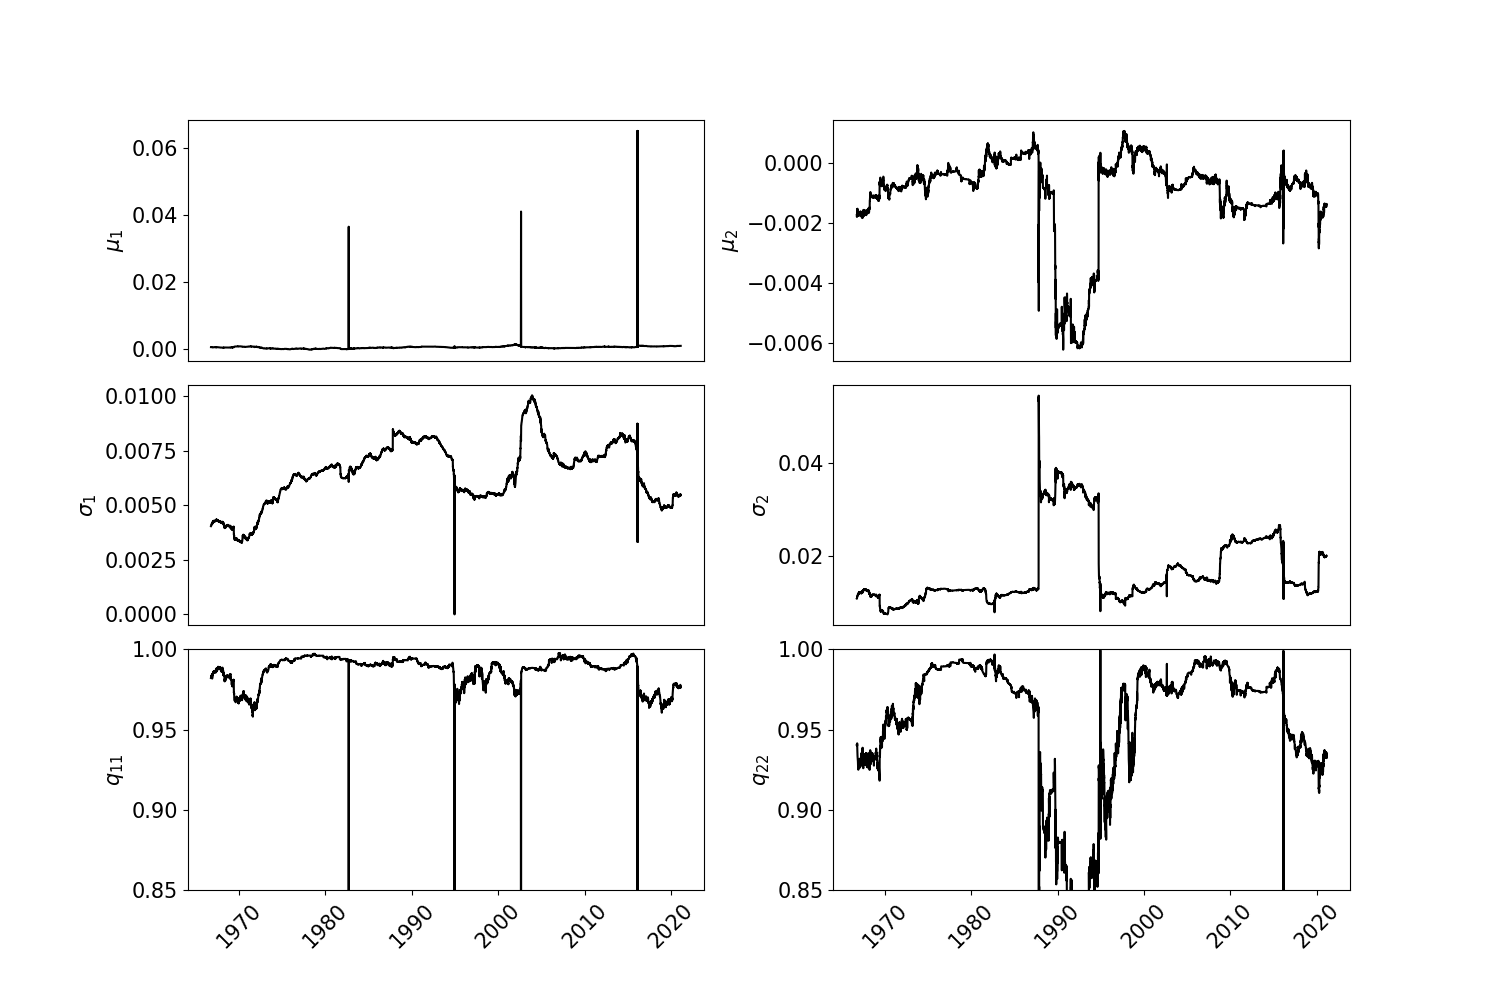
\includegraphics[width=1.0\textwidth]{analysis/stylized_facts/images/2-state MLE HMM rolling params.png}
    \caption[Rolling estimation based on the \mle estimator]{Rolling estimation based on the \mle estimator. Parameters from a 2-state Gaussian HMM using a rolling window of 1700 days. The size of the estimation window is particularly visible in the high-variance state where $\sigma_2$ significantly increase after the financial crisis, and only drops back down to pre-crisis levels after approximately 1700 days.}
    \label{fig: MLE estimation rolling parameters} 
\end{figure}

From figure \ref{fig: MLE estimation rolling parameters} and \ref{fig: Jump estimation rolling parameters} it is evident that neither the mean nor variance parameters exhibit stationarity across time regardless of whether the estimation procedure relies on \mle or \jump. Starting with the \mle approach shown in \cref{fig: MLE estimation rolling parameters}, the rolling window length of 1700 observations is particularly visible in the high-variance state during recessions. This is especially evident during Black Monday in 1987 and during the financial crisis in 2008, in which $\sigma_2$ spikes and doesn't returns to its old level until roughly 1700 trading days later. This is an interesting behaviour, because, as mentioned the most extreme observations from Black Monday and the financial crisis is reduced to plus/minus six times their standard deviation. Yet, during these periods many other extreme returns take place, which is what is responsible for the general change in $\sigma_2$. What's even more interesting is, that both periods of increased variance in $\sigma_2$ lies at roughly the same level. This could imply that the high-variance state fluctuates around some long-run level, in which large deviations only occur for extreme events such as the financial crisis and the COVID-19 recession. It could also imply the need for a third 'outlier' state with a low unconditional probability to handle these periods, but as shown by Bulla (2011) such a model is in some periods inferior to two-state models and does not lead to smaller variations.

Interestingly, figure \ref{fig: MLE estimation rolling parameters} reveals that the mean for the first state is largely time-varying, and with a large notable increase during the financial crisis. The same is true for the mean in the high-variance state, especially during periods of economic turbulence. Thus, the model provides a good estimation for the mean in both states. When analysing the non-constant transition probabilities resulting from the \mle approach in figure \ref{fig: MLE estimation rolling parameters} it can easily be inferred that the sojourn times are mostly persistent in the low-variance state. Contrary, the transition probabilities $q_{22}$ of the high-variance state, are characterised by a higher degree of fluctuations across time, mostly evident during the period follow Black Monday and the big market correction in 2016. This means that the HMM will predict much shorter sojourn times in the high-variance state. This is a natural consequence of the properties of the transition probabilities because when $q_{22}$ decreases $q_{21}$ increases as $q_{22} + q_{21} = 1$, hence a low value of $q_{22}$ will result in more frequent transitions between states.

Moving on to \cref{fig: Jump estimation rolling parameters} it is evident that this methodology also captures the time-varying nature of the underlying HMM parameters. The results are quite similar to those of the \mle estimator, though $\mu_1$ is now practically zero, and the fluctuations in the high-variance state is more abrupt during periods such as Black Monday and the financial crisis than with the \mle estimator. Still, outside periods of economic turbulence, the high-variance state seems more stable with the \jump estimator. Again, the rolling windows are quite clear, for instance, $\sigma_2$ again spikes during Black Monday after which the parameter stabilizes at a new level, only to fall down to its original previous level approximately 1700 days after the event. Curiously though, this time the levels of Black Monday and the financial crisis is not roughly equal, thus rejecting the idea of two long-run levels in $\sigma_2$ - at least for the \jump estimator. 

The biggest improvement of running the \jump framework as opposed to the \mle approach is seen through the estimation of the transitions probabilities for both states. Just as in the simulation study, when comparing $q_{11}$ and $q_{22}$ in \cref{fig: MLE estimation rolling parameters} to \cref{fig: Jump estimation rolling parameters} it appears that the transitions probabilities are much more stable across states when estimating the model parameters using the \jump approach. Furthermore, it appears that both model estimation procedures suggest a similar level for some of the parameters. For instance, $\sigma_1$ generally fluctuates around a level of 0.005 to 0.010 for both approaches. This provides a high degree of confidence since it is more unlikely that two very different estimation procedures should arrive at similar parameters randomly. Conclusively, by analysing figure \ref{fig: MLE estimation rolling parameters} and \ref{fig: Jump estimation rolling parameters} it appears that the \jump approach provides the persistent transition probabilities across time, thereby suggesting that its the strongest methodology, however, further analysis of the reproduction of the stylized facts have to be conducted before this can be cemented.

\begin{figure}[H] 
    \centering
    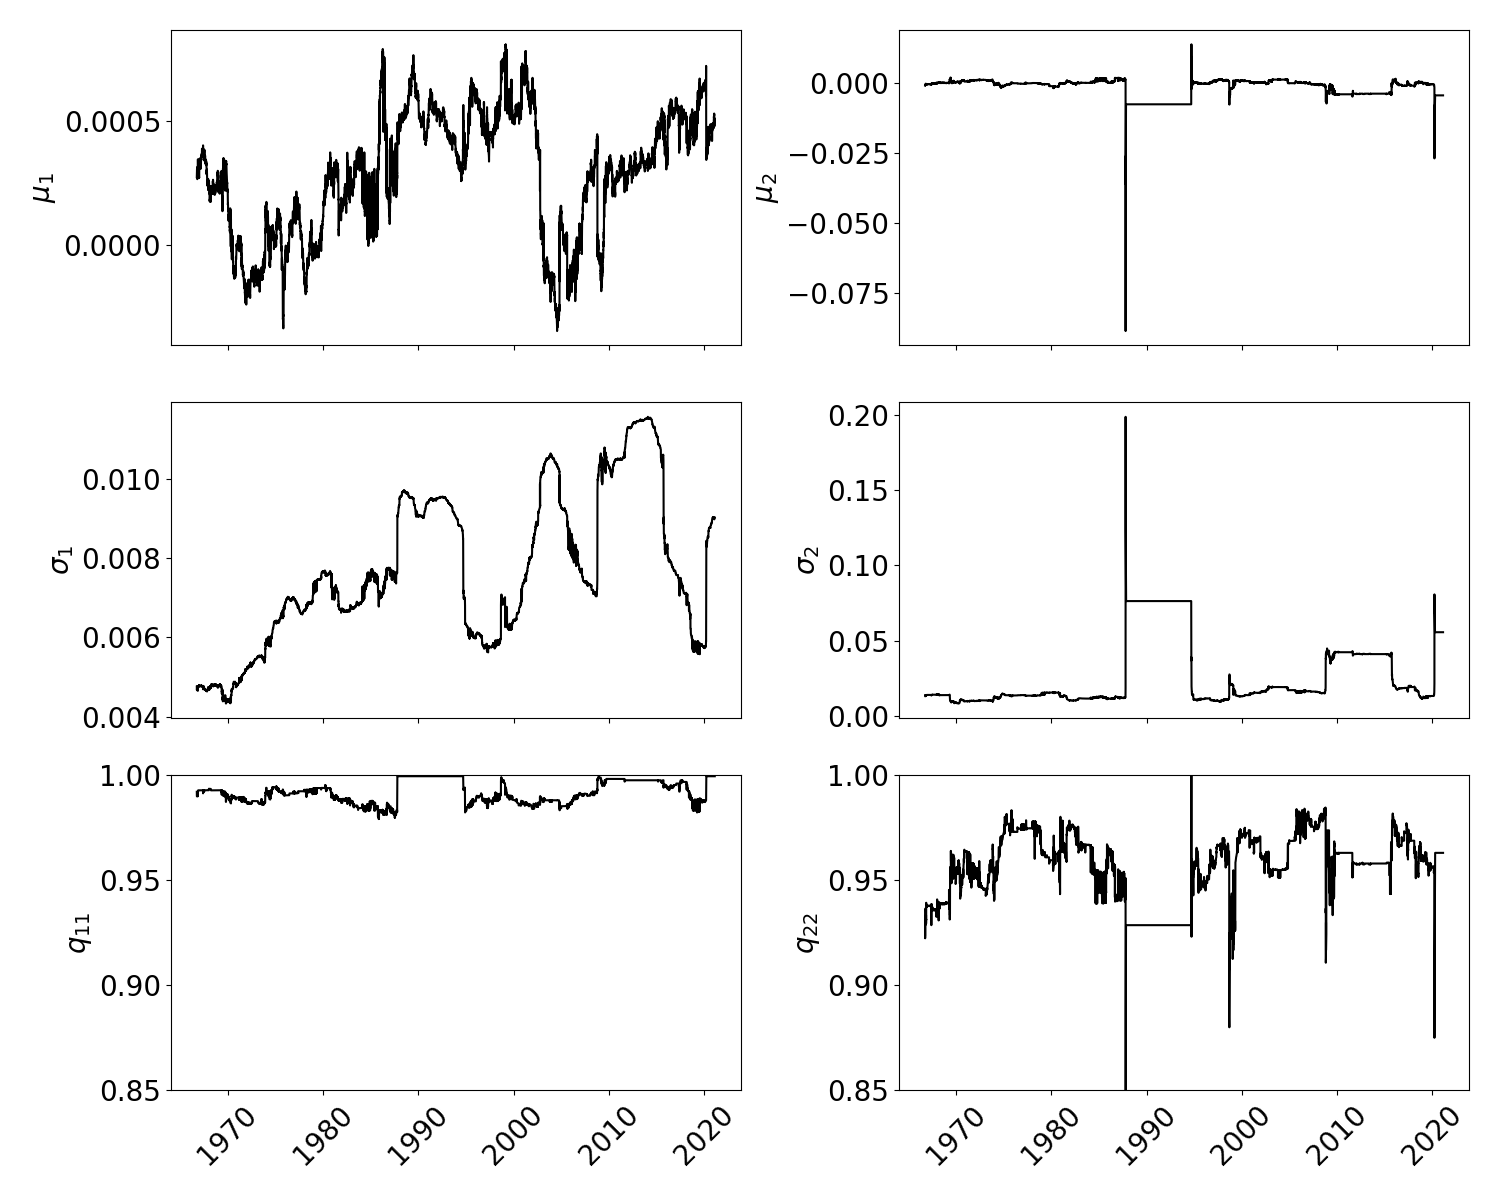
\includegraphics[width=1.0\textwidth]{analysis/stylized_facts/images/2-state JUMP HMM rolling params.png}
    \caption[Rolling estimation based on the \jump estimator]{Rolling estimation based on the \jump estimator. Parameters from a 2-state Gaussian HMM using a rolling window of 1700 days.}
    \label{fig: Jump estimation rolling parameters} 
\end{figure}

Finally, \cref{fig:stylized_facts_rolling_moments} shows the estimated unconditional first four moments of the $r_t$ as well as the \jump and \mle estimators. When analysing \cref{fig:stylized_facts_rolling_moments} it is evident that both the \mle and \jump model are able to reproduce the first two moments quite well, since the mean and variance matches that of $r_t$ across all time periods.

\begin{figure}[H] 
    \centering
    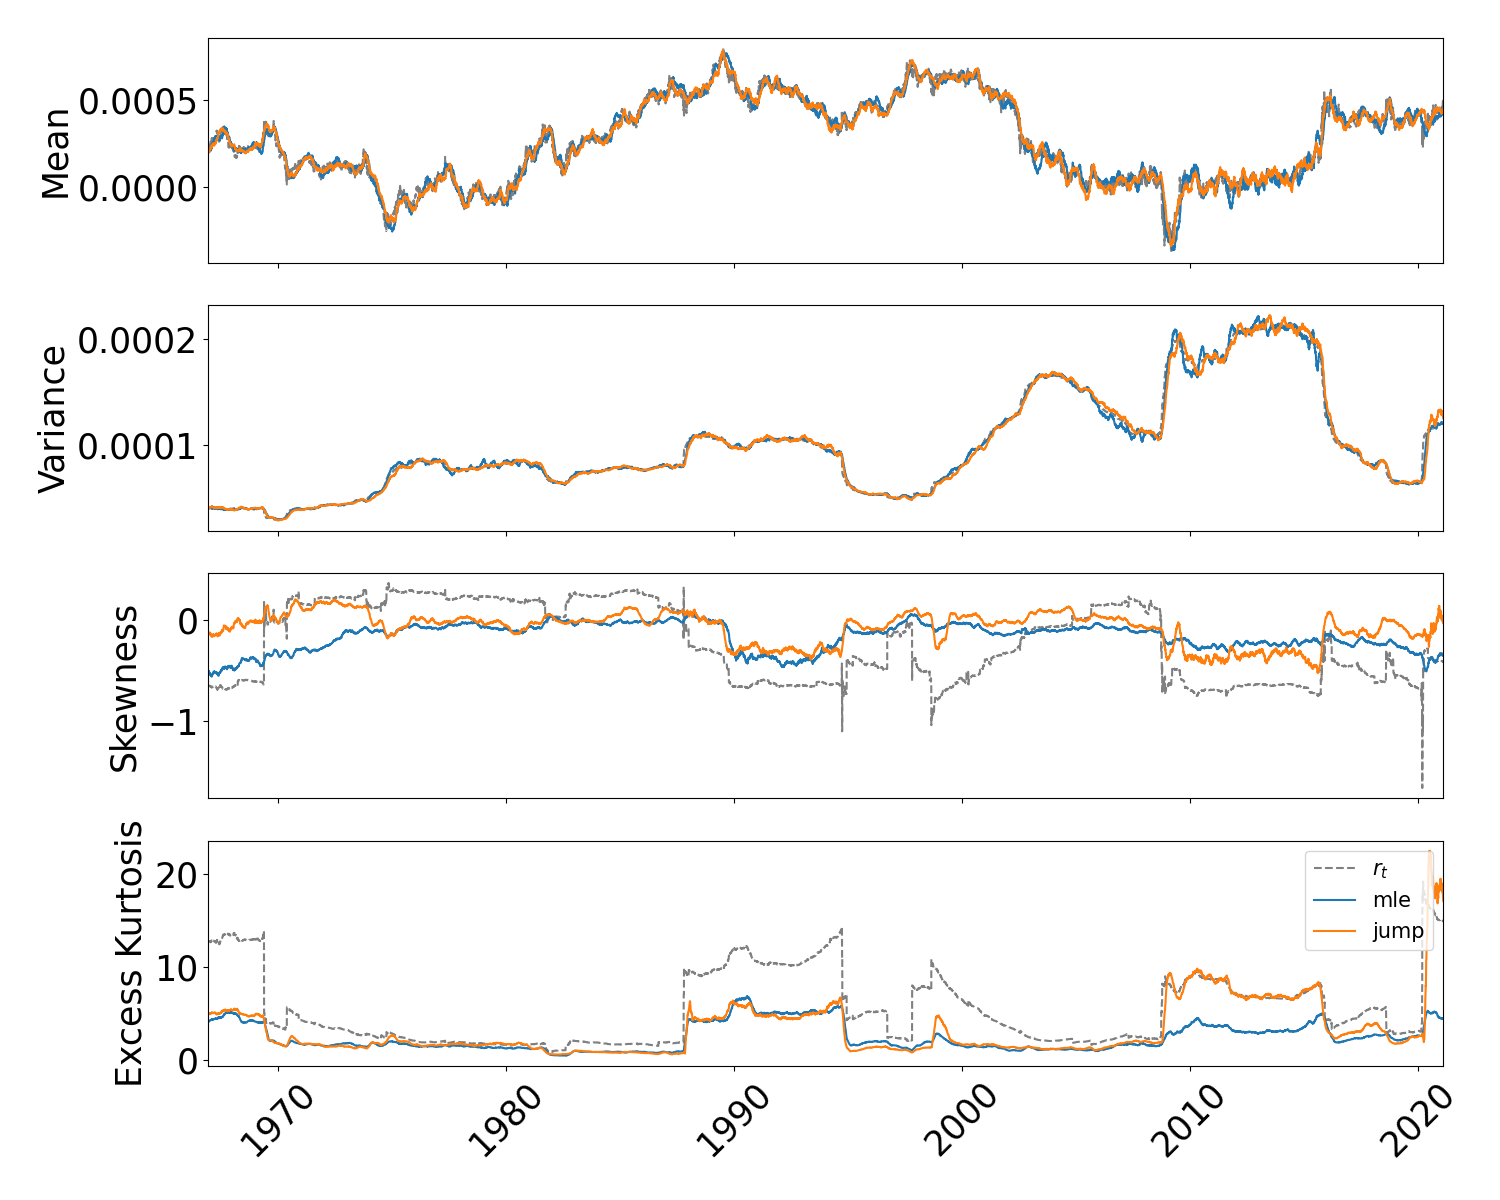
\includegraphics[width=1.0\textwidth]{analysis/stylized_facts/images/moments_regular.png}
    \caption[Development of the first four moments from the estimated models and $r_t$]{Development of first four moments from the estimated models compared to $r_t$ using a rolling window of 1700 days. Model estimates are calculated using Monte-Carlo simulations.}
    \label{fig:stylized_facts_rolling_moments} 
\end{figure}

Unsurprisingly, the estimates of skewness and kurtosis is more error-prone especially during periods of economic turmoil such as during Black Monday. Still, the results are quite similar to those obtained by Bulla (2011) except that we are able to show the full evolution of parameters over the period. Generally, for skewness, the model parameters fluctuates around that of the data, and is predominantly negative during the entire period. This suggest that more observations fall into the left part of the distribution. The same conclusion is apparent for the excess kurtosis where both models' estimates fluctuate around those of log returns. Curiously, Bulla (2011) tended to 'overshoot' kurtosis in many of his 10 subperiods when using t-distributions whilst blaming HMMs using normal distributions for not being able to capture higher levels of kurtosis. It is then interesting to see that, apart from Black Monday, that the \jump estimator is doing a particularly good job of fitting kurtosis, especially during the financial crisis. Additionally, the time-varying nature of the first four moments in \cref{fig:stylized_facts_rolling_moments} further cements the appropriateness in using rolling estimations as a static model would not have been able to capture this observed apparent non-stationary data generating process.

\subsection{Stylized facts of Granger \& Ding (1995b)}
\label{section:stylized_facts_GD}

As the rolling models' parameters have been shown, we now turn to briefly defining the stylized facts established by Granger \& Ding (1995b) before moving on to attempting to reproduce them, in line with Ryden et al. (1998) and Bulla (2011). The temporal properties, established by Granger \& Ding (1995b) are as follows: 

\textbf{Tekst efter TPx skal indentes \newline}
TP1: Returns $r_t$ are not autocorrelated (except for, possibly, at lag 1). \newline
TP2: $|r_t|$ and $r_t^2$ are the 'long memory' i.e. their autocorrelation functions decay slowly starting from the first autocorrelation and $corr(|r_t|, |r_{t-k}|) > (r_t^2, r^2_{t-k})$. The autocorrelations remain positive for many lags and the decay is much slower than the exponential rate of a typical ARMA model. \newline
TP3: The Taylor effect $corr(|r_t|, |r_{t-k}|) > corr(|r_t|^{\theta}, |r_{t-k}|^{\theta})$, $\theta \neq 1$. Autocorrelations of powers of absolute returns are highest at power one. \newline
TP4: The autocorrelation of $sign(r_t)$ are negligibly small.

The three distributional properties are as follows

\textbf{Tekst efter DPx skal indentes \newline}
DP1: $|r_t|$ and $sign(r_t)$ are independent\newline
DP2: $|r_t|$ has the same mean and standard deviation \newline
DP3: The marginal distribution of $|r_t|$ is exponential (after outlier correction)

In addition, it should be noted that an exponentially distributed variable (DP3) $x_t$ has the following properties

PED1: $E(x_t) = \sqrt{Var(x_t)}$ (Same as DP2) \newline
PED2: $E[x_t-E(x_t)]^3 / (Var(x_t))^{\frac{3}{2}} = 2.$ \newline
PED3: $E(x_t-E(x_t))^4 / (Var(x_t))^{2} -3 = 6.$

In the analysis conducted by Rýden et al. (1998) and Bulla et al. (2011) it has been proven that DP1 holds as a natural consequence of the construction of HMMs and that TP1 \& TP4 is not violated in practice. Since DP1, TP1 and TP4 have previously been very well reproduced we don't expect our models to deviate too much from these stylized facts either. The more difficult facts to reproduce, as mentioned, is DP2, DP3, TP2 and TP3, which both Ryden et al (1998) and Bulla (2011) had difficulty in reproducing. It will the analysis of those facts that are most interesting in this study.

In the following two sections we will attempt to reproduce the stylized facts above, starting with the distributional properties and then the temporal ones.

\subsection{Distributional properties}
\label{Sec: Distributional properties}

In this section we shall attempt at reproducing the distributional properties DP2 and DP3, as shown in \cref{fig:stylized_facts_moments_bulla_abs}, which presents the mean-standard deviation ratio, skewness and excess kurtosis of $|r_t|$ and fitted models. In analyzing the ratio of the mean and standard deviation (DP2/PED1), it can be seen that the mean is higher than the standard deviation for the predominant part of the period. This holds for both models, as well as $|r_t|$ although log returns experience larger declines in the ratio during periods of economic turbulence. Therefore, it appears that neither of the two models sway too far away from 1, thereby indicating that the mean of the absolute returns is approximately equal to the standard deviation of the absolute returns for both models. Both \mle and \jump models seem to fluctuate in the interval 1.0 to 1.25, in accordance with Ryden et al. (1998) who noted that PED1 has to be relaxed somewhat, i.e. we have to allow the mean to be slightly larger than the standard deviation.

\textbf{We need a better explanation for why the models might underestimate skewness in most of the period.}

Having analysed whether the models satisfy PED2+DP2 the final distributional property to consider is PED2 and PED3 in DP3. For DP3 to be satisfied the models must exhibit the properties of PED1, PED2 as well as PED3. Since it was just shown that DP2 holds for both models, and PED1 and DP2 is identical in their construction, it can be concluded that PED1 holds for both models. It is evident that both the \mle and \jump model underestimate skewness in most of the period, however, it appears that the \jump model achieves a much better fit of skewness in the period following the financial crisis of 2008. Interestingly, it is clear in \cref{fig:stylized_facts_moments_bulla_abs} that the \mle model better matches the skewness property of PED2 (i.e. that it equals 2) compared to not only the \jump model but also the data $|r_t|$ itself. It should be noted though, that the original DP3 and thus PED2, by Granger \& Ding (1995b) only holds for outlier corrected data, for which the property generally seem to hold for both models and log returns as shown in \cref{fig:stylized_facts_moments_bulla_abs_outliers}. This will be analyzed further in the end of this section.

Still, it appears that both models are able to capture the changing skewness and excess kurtosis around the time of large market movements. This is evident throughout the figure, but particularly around the time of the GFC. The fact that both models are able to do so is particularly promising as it provides substantial evidence towards the adequacy of the models. The fit of the models could be further improved by increasing the number of states, however, the problem with such an option is that it significantly increases the risk of overfitting (Bulla et al. 2011). As such, it can be concluded that both models reproduce these stylized facts quite well.

\textbf{Consider shrinking the y-axis for kurtosis.}
\begin{figure}[H] 
    \centering
    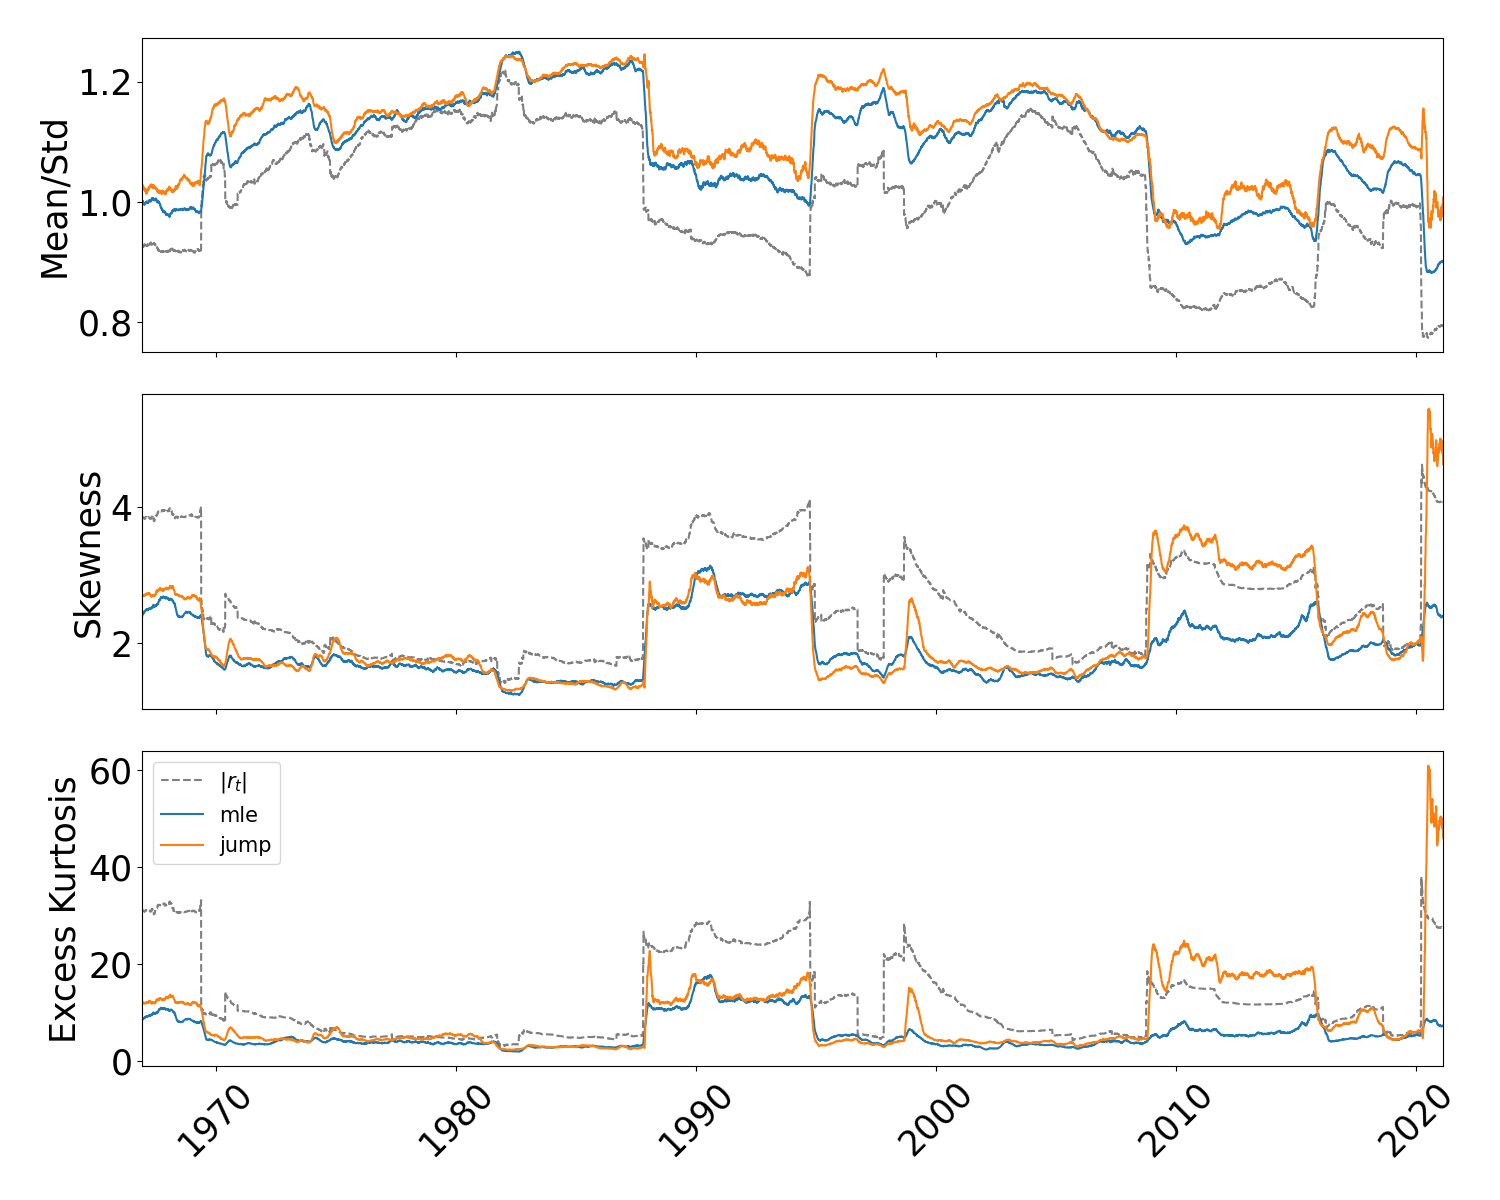
\includegraphics[width=1.0\textwidth]{analysis/stylized_facts/images/moments_bulla_abs.png}
    \caption[Plot of $r_t$ and the models' distributional properties]{Plot of $r_t$ and the models' distributional properties. The first plot shows the mean to std ratio, the middle plot shows the skewness and the final plot shows the excess kurtosis.}
    \label{fig:stylized_facts_moments_bulla_abs} 
\end{figure}

The final property that the models must satisfy in order for DP3 to be met is PED3. As such, the models must be able to exhibit and match an excess kurtosis of 6. It is clear from figure \ref{fig:stylized_facts_moments_bulla_abs} that the \mle model slightly underestimate the excess kurtosis for the predominant time, however, similar to the observations of the skewness, it appears that the \mle model approximately matches an excess kurtosis of 6 in most of the period (its average over the period is 5.51). The \jump model, however, fluctuates around the kurtosis of $|r_t|$ with it being smaller during Black Monday, but slightly larger during GFC and much larger during the Covid-19 outbreak. This is in line with the \jump models slightly larger fluctuation in its parameter estimates of $\mu_2$ and $\sigma_2$ compared to the \mle model. This is quite a satisfactory results as both Ryden et al. (1998) and Bulla (2011) underestimated kurtosis of gaussian HMMs in all their studied time periods.

To summarize the above findings, both the \mle and the \jump models are able to somewhat reproduce the properties of PED1 to PED3, hence it can be concluded that DP3 holds approximately. This is similar to the conclusion reached by both Rýden et al (1998) and Bulla et al. (2011), although they only tested HMMs estimated through the \mle methodology. As such, this section contributes to the quantitative finance literature by showcasing that the stylized facts introduced by Granger \& Ding (1995b) can in fact also be reproduced by a \jump model and not just the traditional HMM estimated through the \mle approach. As such, the thesis have extended on the introduction of \jump estimation procedure for HMMs by Bemporad el at. (2018) by proving that it matches the properties of the stylized facts associated with returns on financial assets.

\subsubsection{Outlier-corrected data}

As a final remark on the distributional properties, we shall examine outlier corrected data limited to the boundary of the closed interval $[\bar r_t - 4\hat\sigma, \bar r_t + 4\hat\sigma]$. As noted by Granger \& Ding (1995b), DP3 was found to only hold on outlier corrected data. Though the above findings where somewhat satisfactory, we repeat the analysis for outlier corrected data. Results are shown in \cref{fig:stylized_facts_moments_bulla_abs_outliers}. Our results are similar to those of Bulla (2011), who didn't find large changes in the results. The mean to standard deviation ratio has risen in magnitude, but the shapes remain largely unchanged. The same conclusion holds for skewness and kurtosis. As a result, the major difference is simply that results have shifted towards the values of an exponential distribution (PED1-3), but the shapes of the curvatures remain roughly unchanged.

\textbf{Begge modeller er her meget tættere på $|r_t|$ end for ikke outlier-corrected data. Men det er kun fordi momenterne har taget et lodret skift ned. Spørgsmålet er om outlier-corrected data vil give bedre density forecasts i den efterfølgende porteføljeøvelse?}

\begin{figure}[H] 
    \centering
    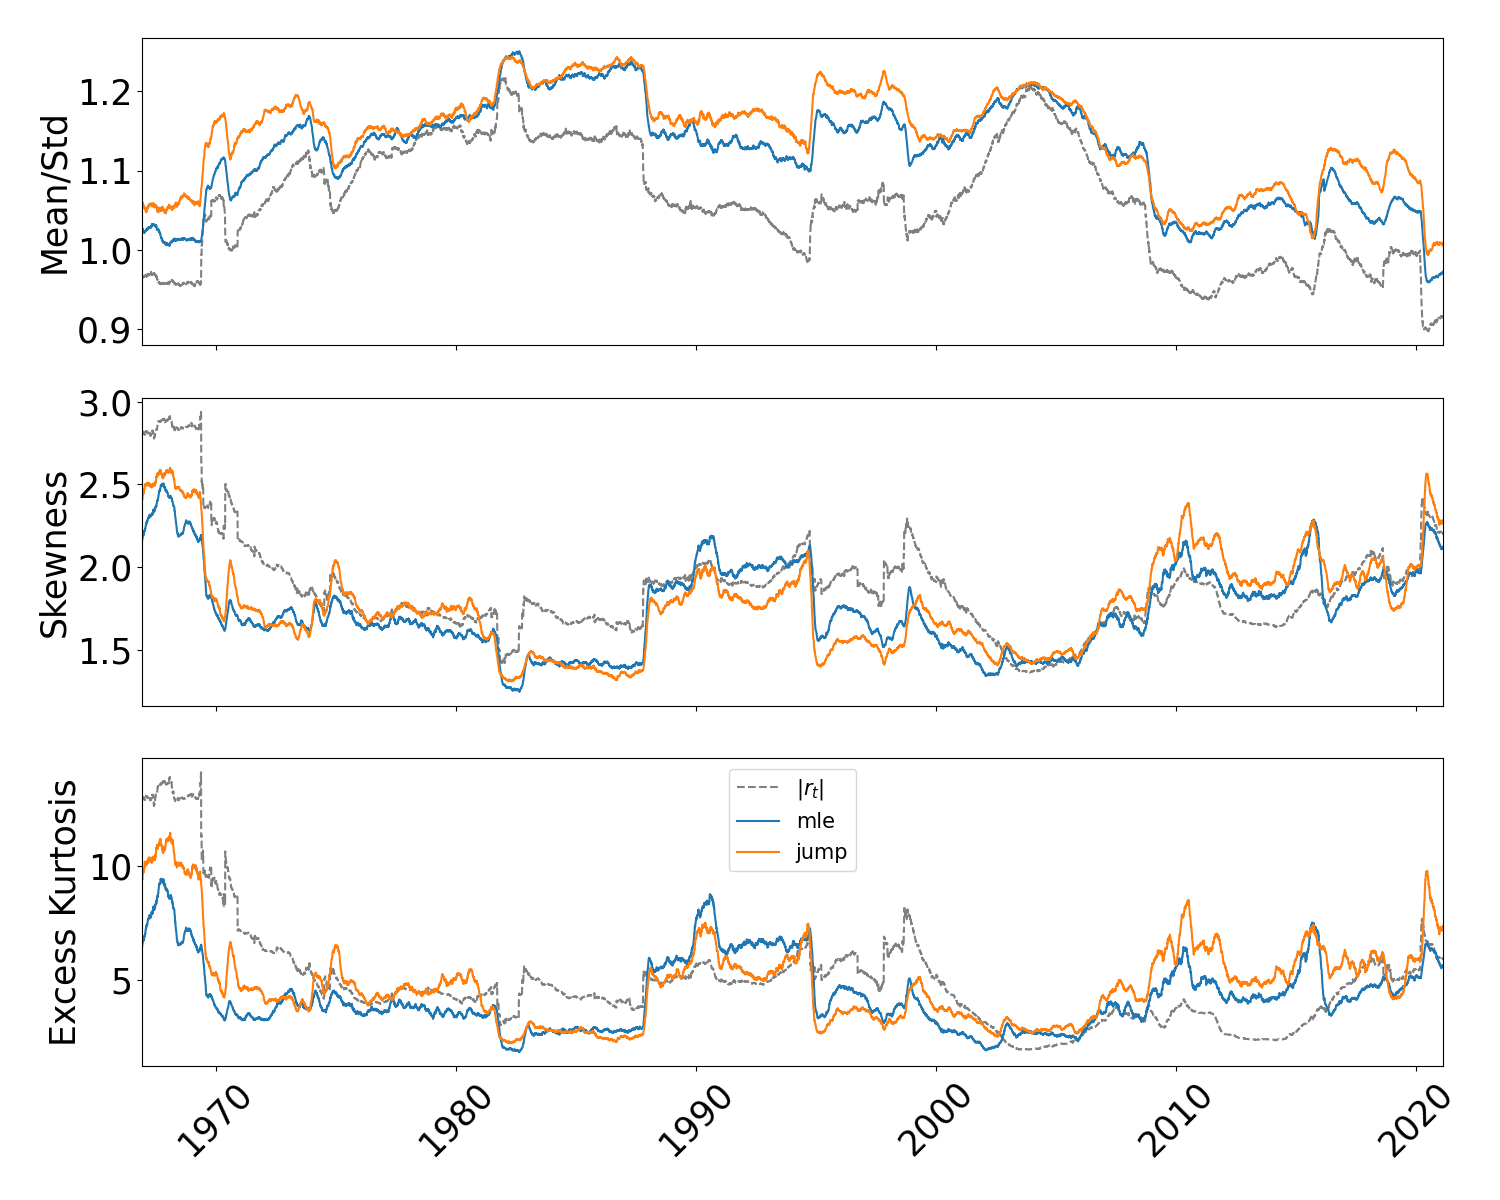
\includegraphics[width=1.0\textwidth]{analysis/stylized_facts/images/moments_bulla_abs_outlier.png}
    \caption[Plot of $r_t$ and the models' outlier corrected distributional properties]{Plot of $r_t$ and the models' outlier corrected distributional properties. The first plot shows the mean to std ratio, the middle plot shows the skewness and the final plot shows the excess kurtosis. \textbf{Consider moving to appendix}}
    \label{fig:stylized_facts_moments_bulla_abs_outliers} 
\end{figure}

\subsection{Temporal properties}
\label{Sec: Temporal properties}

Having analyzed the distributional properties, the next logical step is to check the temporal properties. As mentioned earlier, previous research suggests that HMMs are able to reproduce most of the stylized facts quite well, however, Rýden et al. (1998) and Bulla (2011) found that HMMs are inadequate when it comes to reproducing the slow decay of the autocorrelation function of absolute daily returns which is often referred to as volatility clustering. Ryden et al (1998) this is considered the most difficult stylized fact to reproduce with an HMM.

Thus, most of this section will be dedicated to the reproduction of TP2, though TP3 will also be covered. TP1 and TP4 are shown in \cref{appendix:sign_rt}. The section is structured as follows. Initially, we provide some initial thoughts into why both Ryden et al. (1998) and Bulla (2011) might have had difficulty in reproducing the slow decay in the autocorrelation function. We then show how our rolling models has a much slower decay in their absolute autocorrelation functions when compared to the models of Ryden et al. (1998) and Bulla (2011). Then TP3 is sought reproduced by the \mle and \jump models. Finally we briefly show that TP1 and TP4 is not violated.

\subsubsection{Preliminary thoughts on static versus rolling models' ACF}

We here briefly provide some insights into the difference in the autocorrelation of the full sample and subsamples. This is used to further motivate the use of rolling models.
\cref{fig:stylized_facts_acf_data} shows the autocorrelation of $|r_t|$ on the full sample and the average autocorrelation of subsamples of 1700 observations. On subsamples, the decay is much stronger, and by lag 200 the autocorrelations is practically insignificant. It is most likely as a result of those periods without excess risk and economic turmoil causing very low estimates of the ACF, as the volatility clustering is less significant in these periods. In any case, it is clear that the 'long-memory' effect is clearly decreased in the bottom panel of \cref{fig:stylized_facts_acf_data}.

\begin{figure}[H] 
    \centering
    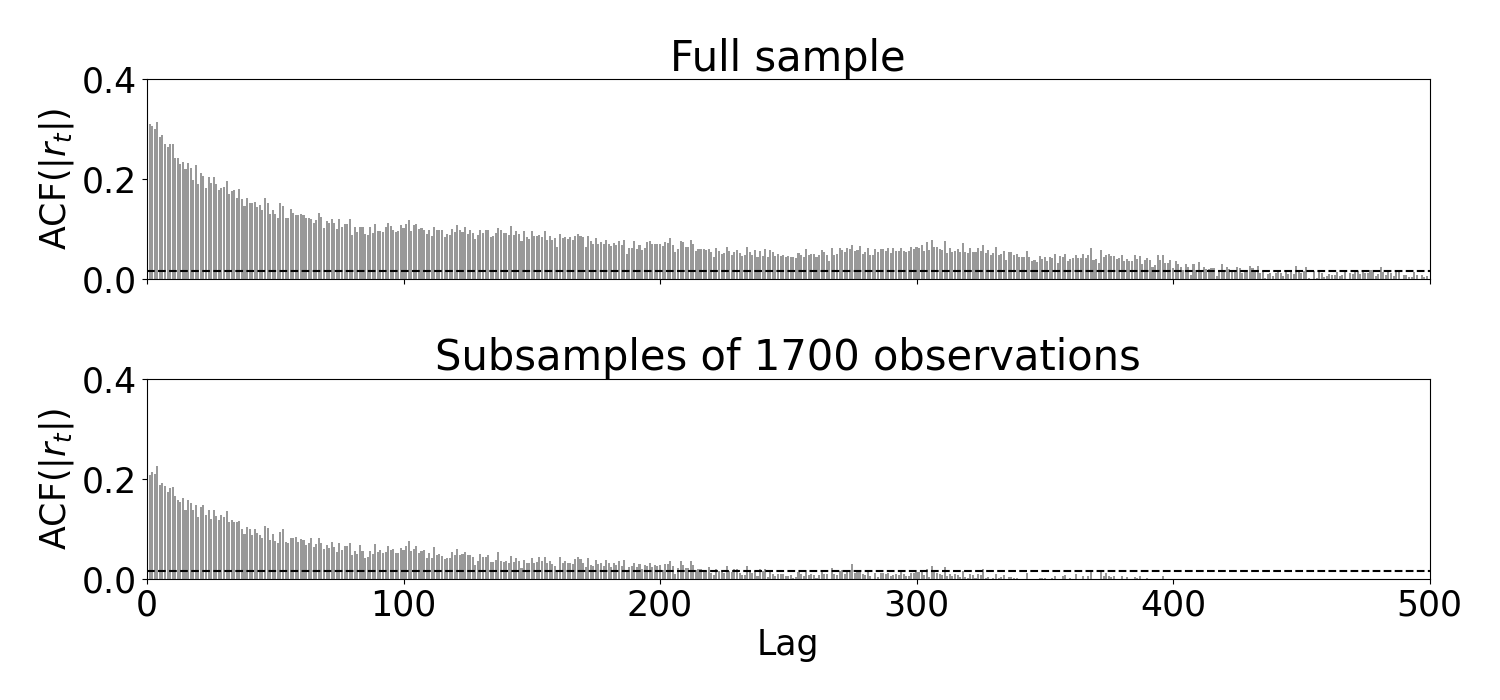
\includegraphics[width=1.0\textwidth]{analysis/stylized_facts/images/acf_data.png}
    \caption[Autocorrelation function of $|r_t|$ on full sample and subsamples]{Autocorrelation function of $|r_t|$. The top panel shows the ACF estimated on the full sample and the bottom panel shows the average ACF when the data is split into rolling subperiods of 1700 observations.}
    \label{fig:stylized_facts_acf_data} 
\end{figure}

This finding should already make one suspicious of estimating static models in a few subsetted periods as Ryden et al. (1998) and Bulla (2011) did. To show the performance of our models in such a setup, we repeat the procedure by Ryden et al. (1998) and Bulla (2011). Results are shown in \cref{fig:stylized_facts_acf_plots_sub_periods}. As mentioned above, there exists clear differences in the level of ACF between the subperiods, with some periods exhibiting quite high levels of autocorrelation, and other periods in which it dies down within 50 lags. The performance of both models \mle and \jump is roughly as reported by Bulla (2011), in which the decay is generally much faster for the models than for log returns. One interesting finding though, is that the \mle model appear to model autocorrelation quite well in periods 3 and 8, which are periods of turmoil. Having shown how our models would have performed in a static scenario, we now repeat the procedure for the rolling model.

\begin{figure}[H] 
    \centering
    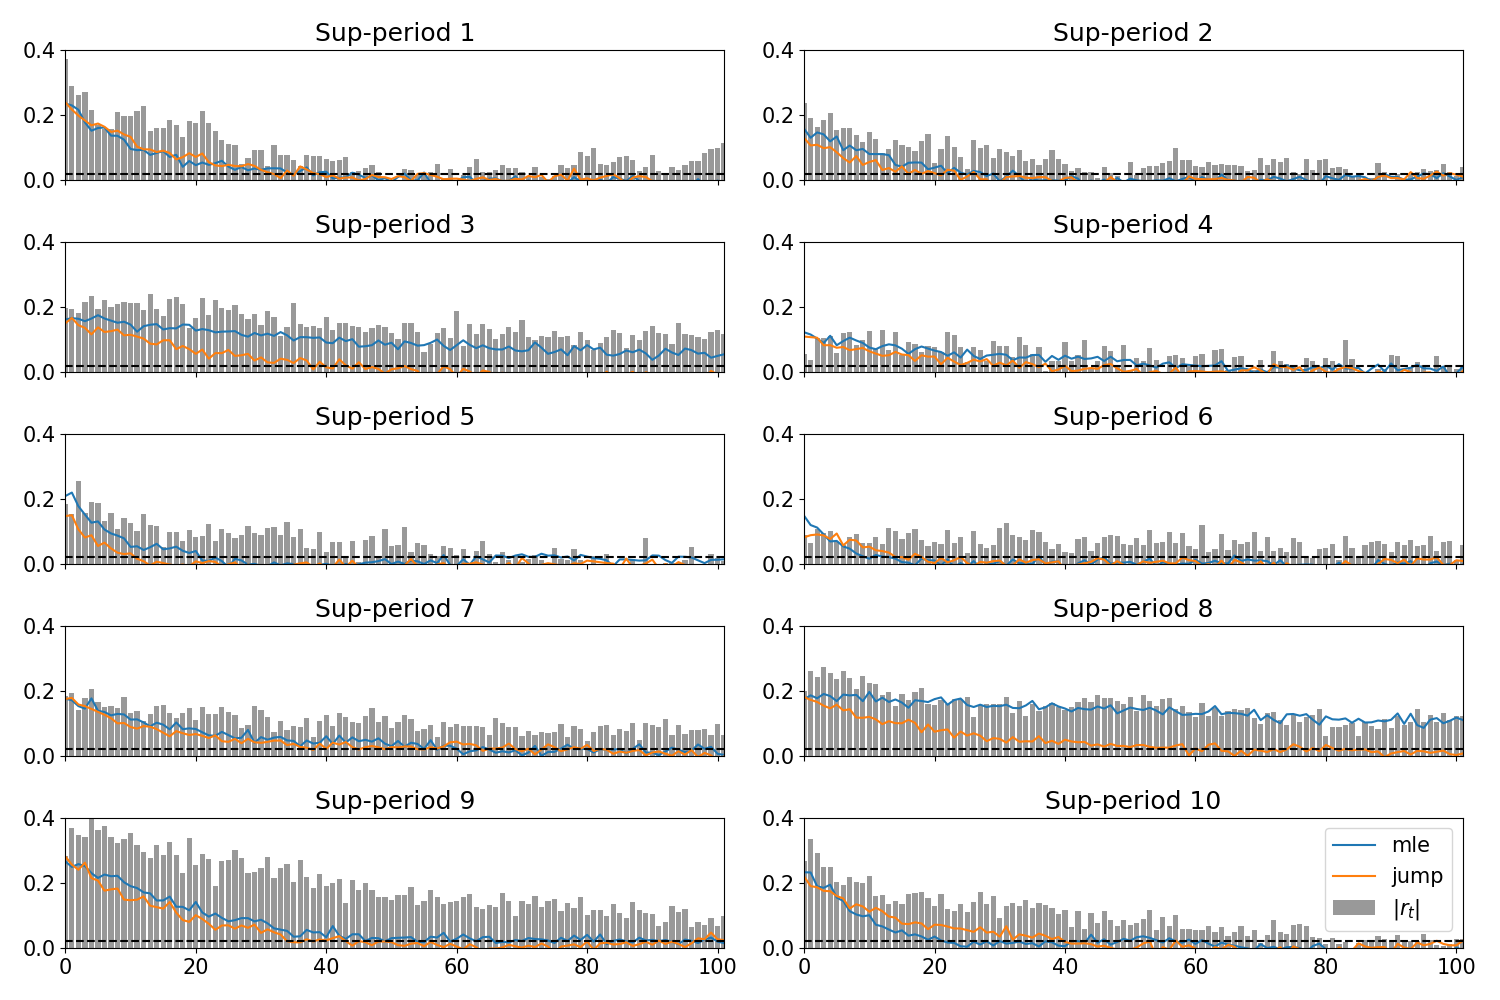
\includegraphics[width=1.0\textwidth]{analysis/stylized_facts/images/acf_abs_subperiods.png}
    \caption[Autocorrelation function of estimated models and $|r_t|$ on subsamples]{Autocorrelation function of estimated models and $|r_t|$ in a breakdown of 10 sub each of 1700 observations. \textbf{Ret stavefejl i Sub-period.}}
    \label{fig:stylized_facts_acf_plots_sub_periods} 
\end{figure}

\subsubsection{Temporal properties of the rolling model}

In order to get an overview for the full sample period figure \ref{fig:stylized_facts_acf_plots} plots the full sample empirical absolute autocorrelation function together with the simulated absolute ACF functions of the \mle and \jump models. The dashed line is the upper boundary of the 95\% confidence interval under the null hypothesis of independence (Madsen, 2008). The autocorrelations of both models \mle and \jump, have significantly increased and is now well above that of the data at lags above 350. Interestingly, the initial decay of both models is stronger than $|r_t|$ for the first $\sim$ 50 lags, after which it flattens out.\textbf{Think about a good reason for why this might be.}
The reader should note that the persistence of the ACF of the absolute returns is, to some extent, a consequence of the aforementioned volatility clustering, and the significant level of the lags above lag 100 is more likely a result of the data-generating process being non-stationary as mentioned earlier. 

\begin{figure}[H] 
    \centering
    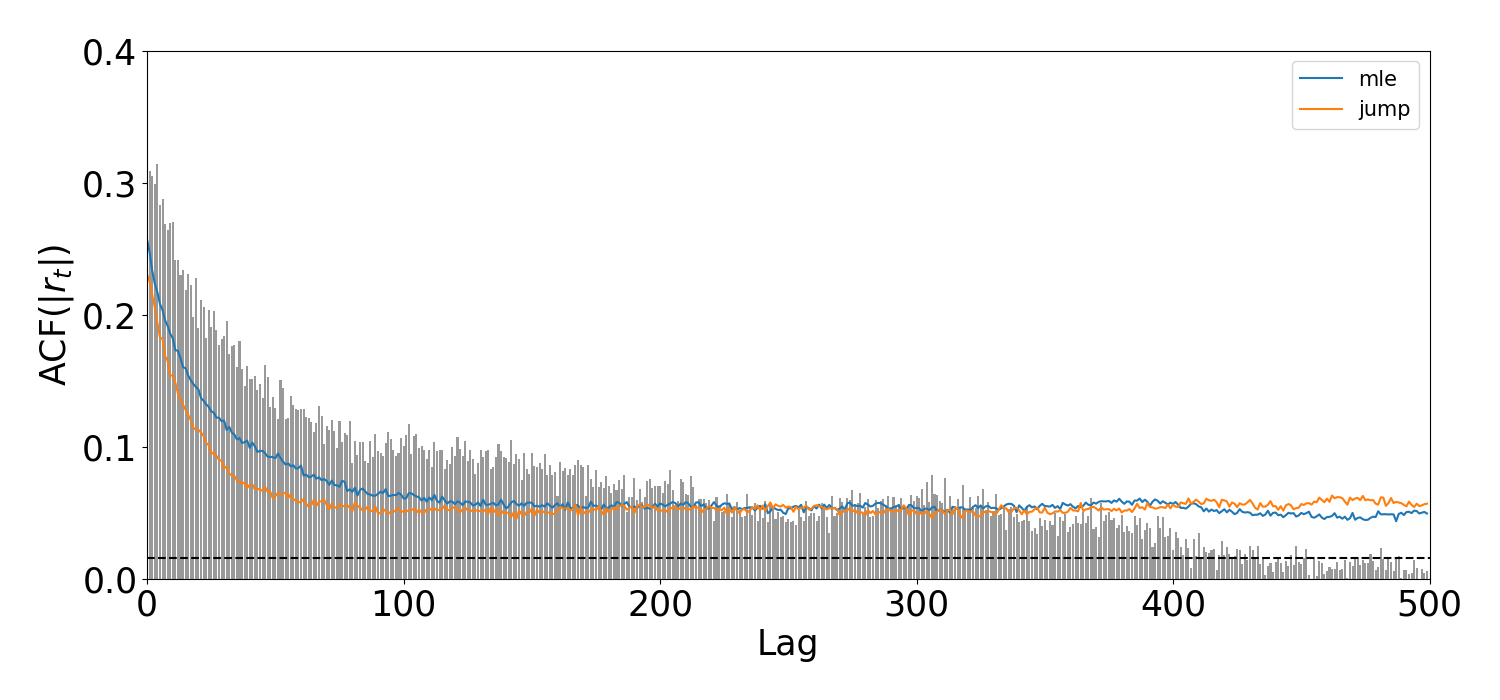
\includegraphics[width=1.0\textwidth]{analysis/stylized_facts/images/acf_abs.png}
    \caption[Autocorrelation function of estimated models as well as $|r_t|$ on full sample data]{Autocorrelation function of estimated models as well as $|r_t|$ on full sample data.}
    \label{fig:stylized_facts_acf_plots} 
\end{figure}

From the plot in figure \ref{fig:stylized_facts_acf_plots} it is evident that that \mle model does a better job at reproducing the shape of the absolute ACF for the first 200 lags, however after that, their performance is similar. In addition, neither of the model's absolute autocorrelation become insignificant even at very large lags, which is in-line with the actual autocorrelation of the absolute empirical ACF. The reader should note, that since the computation underpinning the autocorrelation plots of figure \ref{fig:stylized_facts_acf_plots} relies on simulations, the true autocorrelations are probably higher, as the bouncing behaviour from simulations exhibited in figure \ref{fig:stylized_facts_moments_bulla_abs_outliers}, should reduce autocorrelation.

The remaining stylized fact is TP3, i.e. $corr(|r_t|, |r_{t-k}|) > corr(|r_t|^{\theta}, |r_{t-k}|^{\theta}) \forall \theta \neq 0$, which is often referred to as the Taylor effect. In order to analyse whether the Taylor effect holds, the coefficient $\theta$ is estimated for every period by maximizing the first order autocorrelation of $|r_t|^{\theta}$. As with Rýden et al. (1998), we also perform the computation through Monte-Carlo simulations and subsequent numerical maximization.

\begin{figure}[H] 
    \centering
    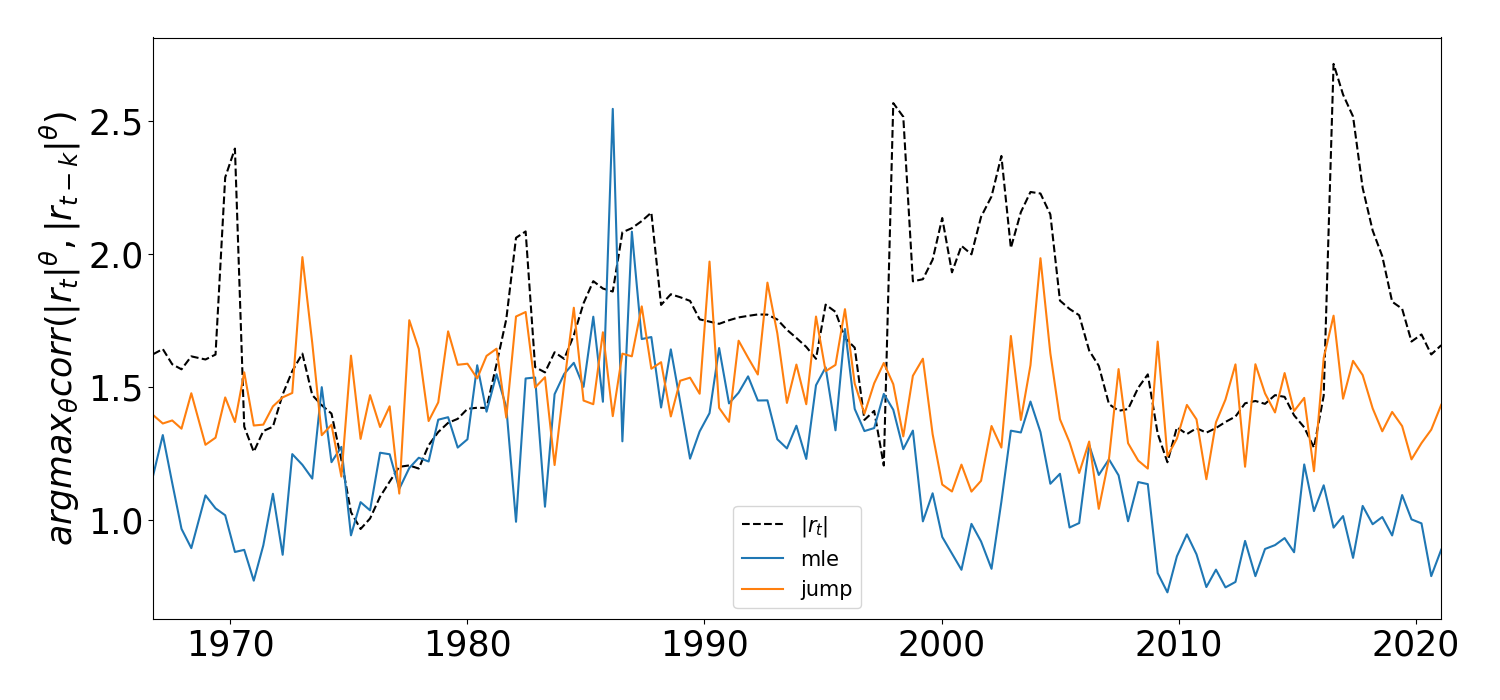
\includegraphics[width=1.0\textwidth]{analysis/stylized_facts/images/taylor_effect.png}
    \caption[Taylor effect comparison of the $\theta$ maximizing first order autocorrelations of $|r_t|^{\theta}$ and for the models]{Taylor effect comparison of the $\theta$ maximizing first order autocorrelations of $|r_t|^{\theta}$ and for the models. It is computed by Monte-Carlo simulations and subsequent use of numerical maximization.}
    \label{fig:stylized_facts_taylor_effect} 
\end{figure}

Figure \ref{fig:stylized_facts_taylor_effect} summarizes the results. On the
one hand, maximizing values of $\theta$ for the data series are are not exactly equal to 1, thereby suggesting that neither models fully captures the properties stipulated by TP3. Even so, the fluctuation of both models is roughly the same as that observed by $|r_t|$, although the data fluctuates more aggressively. Apart from a smaller period from 1998-2005, the general direction of both models generally appear to follow that of the data, indicating model adequacy.

\subsection{Decoding and prediction}

\textbf{This section is currently not really used for anything except showing pretty graphs as state prediction is not used in the asset allocation strategies. Should be changed to either focus on the posterior probabilities in each state, since this is used in forecasting, or something else. Otherwise delete.}

\textbf{Should be centered around 1-step density forecasts or the persistence of states in a rolling model.}

\textbf{Test if state persistence is improved on outlier-corrected data --> This can easily be done in an out-of-sample setting.}


As mentioned in section \ref{section: estimation} the hidden states are uncovered through the Viterbi algorithm. Since the estimation procedure is based on a rolling window, the state at time $t$ is estimated by using the most recent observation as well as the previous 1699. As such, the decoding procedure iterates through the entire row of observations 1 time step at a time as shown in figure \ref{fig:stylized_facts_decoded_states}. As previously mentioned, it is important to stress that the objective of this procedure is not to predict future states of the economy, but rather to identify and uncover the current state underlying the economy given past observations. 

\begin{figure}[H] 
    \centering
    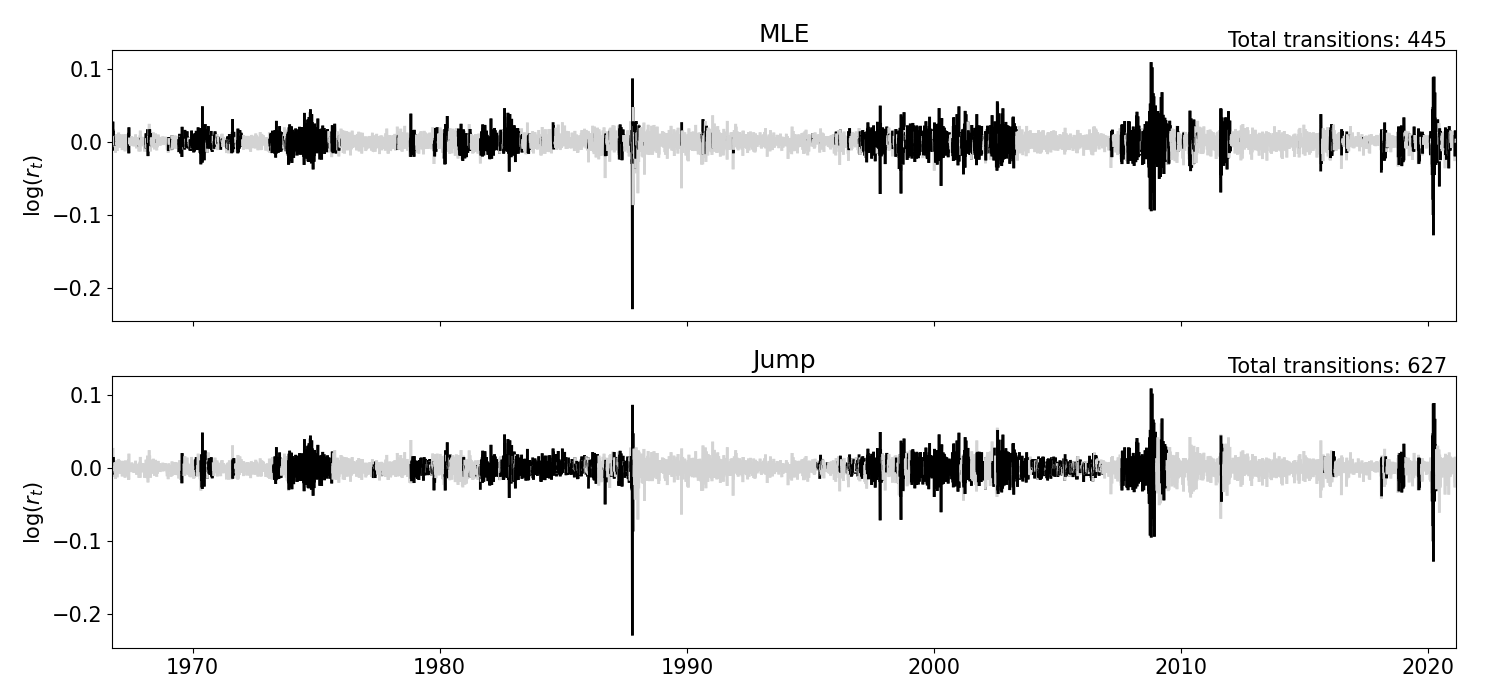
\includegraphics[width=1.0\textwidth]{analysis/stylized_facts/images/decoded_states.png}
    \caption[S\&P 500 $\log r_t$ plotted with the respective models' decoded states]{S\&P 500 $\log r_t$ plotted with the respective models' decoded states. States are decoded using a rolling window of 1700 trading days. Black indicates the high-variance state.}
    \label{fig:stylized_facts_decoded_states} 
\end{figure}

It is evident from the figure that the \mle model does a decent job in detecting the high-volatility states. However, it also appears that the model identifies some high-variance states in periods characterised by low market volatility, for instance in the beginning of the 1990s. This is most likely a result of low excess kurtosis. A similar pattern appears when analysing the decoding states of the \jump model since it too does a fairly good job at identifying the high-variance state, although the two methods disagrees in some time periods. This is for instance evident when looking at 1985 to 1990 where the \mle models suggests a low variance state, contrary to the \jump model. Furthermore, it appears that the \jump model is less consistent compared to the \mle model as it jumps around more sporadically. This is backed by the fact that the \jump model suggests 627 state transitions throughout the period which is more than 40\% more state changes compared to the suggested 445 transitions by the \mle model. This is perhaps surprisingly since the \jump framework penalizes state transitions, however, this is most likely a result of the rolling estimation approach. As such, if one were to conduct a similar analysis in which the \jump model was estimated by batches or on the full sample size, the total suggested transitions would most likely decrease, albeit these estimation procedures would introduce other problems. 

In addition, it is positive to witness that both models correctly identifies major market events such as Black monday in 1987, the dot-com bubble of the early 2000s, the GFC of 2008 and most recently the COVID-19 recession as high-variance states, albeit the models disagree in terms of how long the high-variance state persists. Furthermore, it was evident by figure \ref{fig: SP500_index} that there were short periods of large positive returns following the big market crash in September/October 2008, however, both models predict those as bear states, which indicates that variance dominates means in the prediction of whether a state is classified as high or low variance. Another aspect that has to be considered in terms of using the either model, but particularly the \jump, is the cost of changing the portfolio allocation due to a wrong signal. As evident by figure \ref{fig: SP500_index} the period from 1980 to 1990 is characterised by increasing price levels and low variance, hence the correct classification of the state should be low-variance, however, the \jump model classifies it as a high-variance state throughout the period. As such, utilising the models when forming DAA strategies should be done carefully, as the amount of transitions and possibly miss-specified states can decrease profits and Sharpe ratios substantially.  

\subsubsection{Smoothing}
In the previous section it became evident that the amount of transitions between the two states are high for both models with the \mle and \jump model proposing 445 and 627 transitions respectively. This amount of state transitions decreases the confidence that the uncovered state changes occur due to the economy entering a new state, while increasing the suspicion towards random sporadic jumps. Furthermore, it was evident that the \jump model proposed more than 40\% more transitions compared to the \mle, and this constitutes an issue due to the objective of \jump model being to constrain sporadic and frequent jumps. Lastly, such fluctuations and sporadic transitions can be costly in a DAA framework, especially when factoring in opportunity cost of allocating capital poorly due to a miss-specified state, and when factoring in actual trading costs. As a result of these conclusions, a probability smoothing scheme is implemented to improve persistence and hence reduce the amount of state transitions. For every state prediction at time $t$, the probability of being in all states are computed as described in section \ref{section: estimation}. This is then compared to a median threshold hence a state change will only occur if the past 4 out of 7 state predictions suggest that a change must occur. The choice of threshold is a trade-off between the time-delay in state changes and the confidence in state predictions as described by Nystrup (2014). The associated results of applying such a smoothing scheme is shown for the \mle and \jump model in figure \ref{fig:stylized_facts_decoded_states_filtered}.

\begin{figure}[H] 
    \centering
    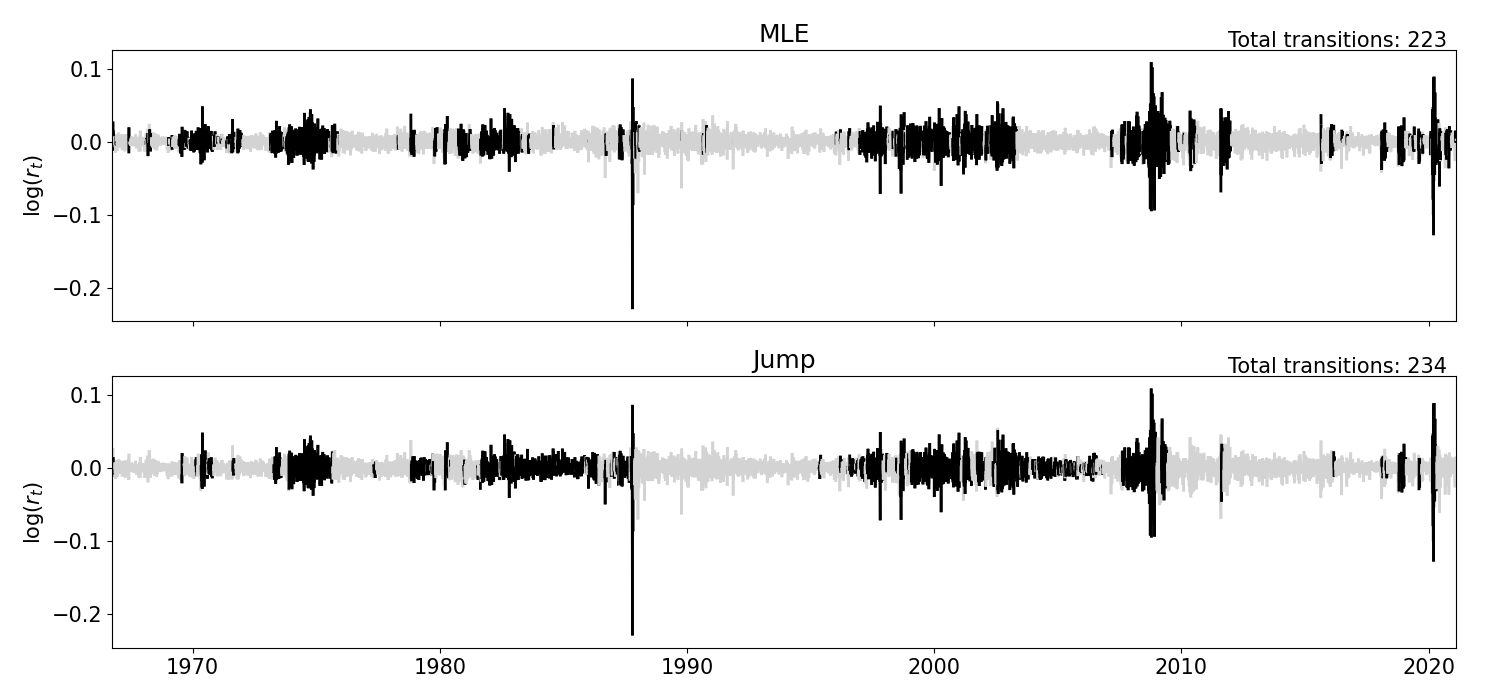
\includegraphics[width=1.0\textwidth]{analysis/stylized_facts/images/decoded_states_filter.png}
    \caption[S\&P 500 $\log r_t$ plotted with the respective models' smoothed decoded states]{S\&P 500 $\log r_t$ plotted with the respective models' smoothed decoded states. States are decoded using a rolling window of 1700 trading days.  Black indicates the high-variance state.}
    \label{fig:stylized_facts_decoded_states_filtered} 
\end{figure}

It is evident that the number of proposed transitions reduces dramatically from 445 to 223 for the \mle model and from 627 to 234 for the \jump model. The drastic decrease in transitions is primarily visible in the fewer amount of short-lived sojourn times. However, despite the apparent decrease in the number of transitions, there still appears to be inconsistency across the two models in terms of state predictions. This is once again evident in the time period from 1985 to 1990 in which the \mle model suggests low-variance states and the \jump model suggests high-variance states. Yet, both models are still able to capture the big market events as previously described. Furthermore, applying the probability smoothed models serve as a better option compared to the non-smoothed alternative in a DAA framework since the reduction in state transitions, all else equal, will reduce trading costs and increase returns. 

As conclusively remarks of section \ref{Section: Stylized facts}, it appears that both the \mle and \jump model are able to reproduce the four temporal as well as the three distributional properties, however, the \jump model does an overall better job. Particularly, when reproducing the empirical absolute autocorrelation function the \jump model achieves a better fit for the first 200 lags, although the \mle achieves a better fit for the remaining lags. Furthermore, there is a significant variation in the parameters over time, thereby greatly supporting the use of rolling estimation. In addition, the use of rolling estimation has the property that no foresight is assumed at any point in time, thereby making the prediction model likely to generalize well to new data. Lastly, a smoothing scheme has been applied when uncovering the hidden states, thereby increasing state persistence while reducing the amount of transitions between states. Despite these initiatives, it is clear that the models still provide inconsistent state predictions thereby increasing the risk of making poor capital allocation decision, and as a result encounter decreasing profits through a DAA framework. In the following sections, the MPC framework will be introduced and based on this it will be investigated whether trading strategies conditional on the predicted states are profitable.
